\documentclass[10pt,a4paper]{article}
\usepackage[margin=17mm]{geometry}
\usepackage[T1]{fontenc}
\usepackage{lmodern,microtype,graphicx,booktabs,amsmath}
\usepackage[hidelinks,pdfauthor={},pdftitle={Computer Graphics - Technical Brief Report}]{hyperref}
\setlength{\parindent}{0pt}\setlength{\parskip}{4pt}
\begin{document}
{\LARGE\bfseries Computer graphics assignments}\par
{\large Technical Brief Report}\par
The collection explores explicit graphics pipelines through Python/OpenGL coursework, a Maya animation scene, and a packaged Unity game. The Python exercises use the Elements teaching framework's entity--component scene graph, NumPy geometry, GLSL shaders, and ImGui controls.
\section*{Geometry, shading, and motion}
\textbf{Assignment 1} builds sphere vertices and indexed triangles, composes object and group translation/rotation/scale matrices, and renders triangle, line, and point primitives. The active sphere entry point displays one wireframe sphere. Additional variants in the submission are commented examples rather than active modes.

\textbf{Assignment 2} separates mesh geometry from shader/material state. Flat normals support the lighting example, with GUI controls for colors, shininess, and light properties. The next scene adds UV coordinates, a textured-sphere shader, two light sources, an orbiting light position, and a cubemap. The Earth mapping remains incorrect: the current rendering is not evidence of a successful Earth texture. The original submission also records a texture defect.

\textbf{Assignment 3} assigns weights to vertices and blends three joint transforms in the vertex shader:
\[M=w_0M_0+w_1M_1+w_2M_2,\qquad p_{clip}=PVM_{model}Mp.\]
Two keyframes interpolate joint angles over a five-second animation loop. Manual angle controls remain available when animation is off. This demonstrates the connection between per-vertex attributes, matrix uniforms, and deformation. The Maya binary scene is a separate artifact. The original submission describes an L-shaped assembly with joints and five keyframes, but that scene was not executed during this review.
\begin{center}
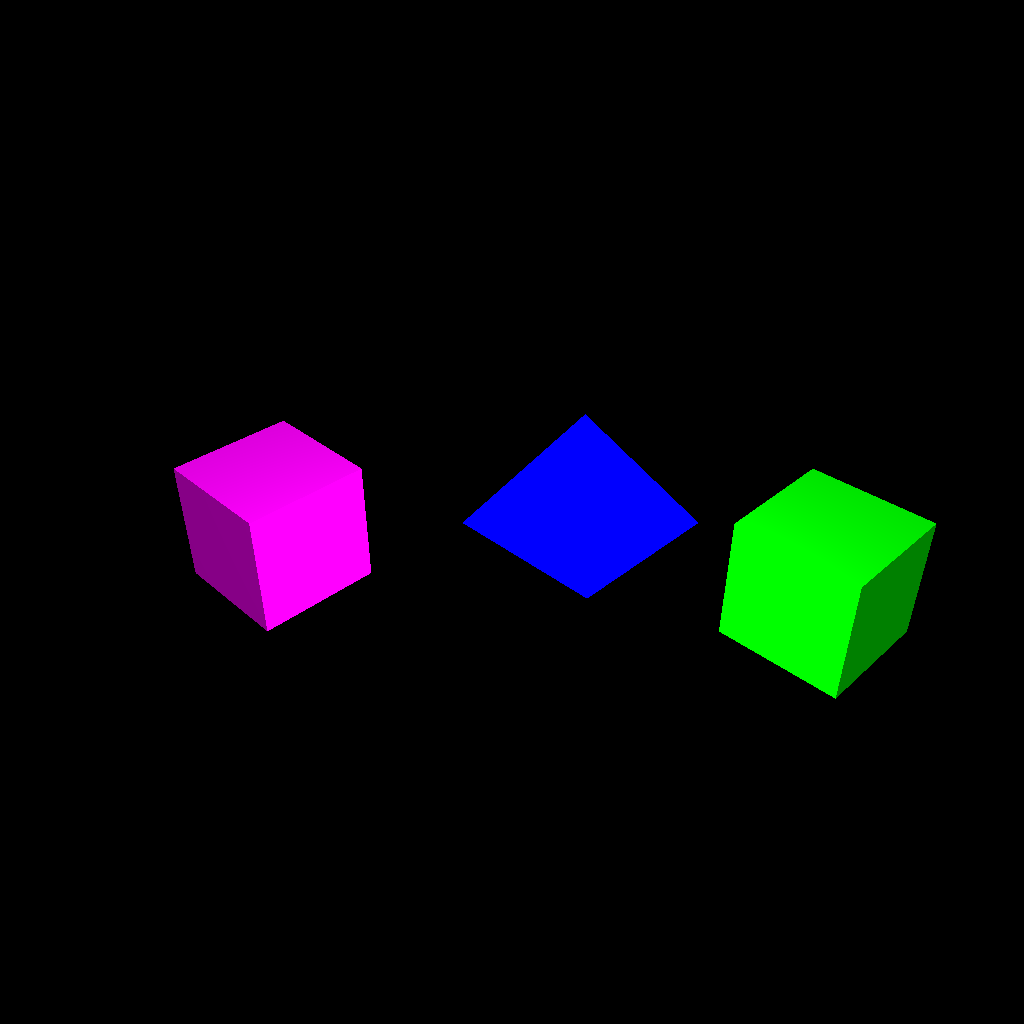
\includegraphics[width=.32\linewidth]{assets/lighting.png}\hfill
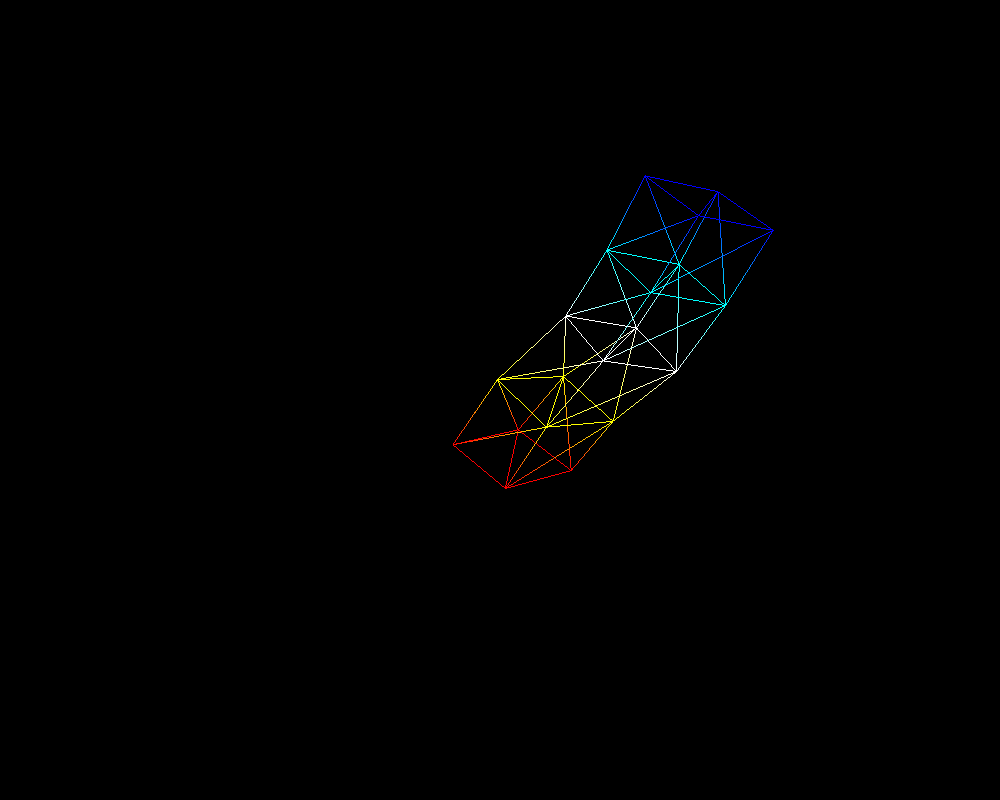
\includegraphics[width=.32\linewidth]{assets/joints.png}
\end{center}
{\small Actual framebuffer captures of the Python lighting and joint-transform scenes, rendered through Mesa software OpenGL before GUI overlays.}
\section*{Execution and reproducibility}
All six Python entry points completed 60-frame capture runs using Python 3.10.22, NumPy 1.26.4, SDL offscreen rendering, and Mesa OpenGL 4.5 via llvmpipe. These runs verify initialization, shader/mesh setup, and the demonstrated rendering paths. They do not exhaustively test GUI interaction or measure hardware performance.

A central launcher selects the exercise and loads the supplied shader extension without overwriting the framework installation. The framework is pinned to commit \texttt{7617f647dee71d9978adca0db0e3a99324f245b3}. Compatibility adjustments update decorator imports and remove an unused Unix-only import. Texture creation occurs after context initialization. A bundled cloudy cubemap replaces missing star images. The rendering algorithms otherwise retain the supplied coursework implementation.

\textbf{Assignment 4} is a Windows Unity 2022.3.22f1 build, including the player, data files, managed assembly, and Mono runtime. Verified split parts reconstruct the original ZIP with one Python command. It does not contain an editable Unity project. Game startup could not be verified here. The separately linked solar-system project is also absent from the supplied archives.

The repository's \href{https://github.com/mitsosasim/graphics_uoc/blob/main/docs/SETUP.md}{PC setup guide} covers every Python command, native GUI controls, Maya opening steps, and extracting/launching the Windows game. Python source credits Dimitrios Asimakopoulos, csd4845. Elements framework code and assets originate upstream and retain their respective terms.
\end{document}
